% ===== 08_xian =====
\section{西安疫情数据应用}
\label{sec:xian}

本节先采用 He、Tang 和 Xiao~\cite{He2023TDINN} 给出的西安疫情 TDINN 控制函数和日报数据，将 $c(t)\equiv c_0$ 的仅隔离阈值策略用于西安参数下的数值计算，并与 TDINN 重构控制及常规控制比较。同一起止状态下的联合阈值分配另见第\ref{sec:joint:compare-numerics}节和表\ref{tab:joint:compare}，并在本节简述其结果。TDINN 控制同时降低接触率、提高隔离率；这里的仅隔离阈值对照则保持接触率不变，仅通过提高隔离率使社区感染者人数 $I(t)$ 不超过 $\eta$。记社区感染者 $I(t)$、新增社区感染 $I_{\rm new}(t)$、新增隔离感染 $I_{q_{\rm new}}(t)$、累计社区感染 $I_{\rm cum}(t)$、累计隔离感染 $I_{q_{\rm cum}}(t)$，以及总累计感染 $\Itcum(t)=I_{\rm cum}(t)+I_{q_{\rm cum}}(t)$。

\subsection{真实数据与 TDINN 控制函数}
病例数据包含社区发现病例数 $I_{\rm new}(t)$ 和隔离发现病例数 $I_{q_{\rm new}}(t)$，覆盖 2021 年 12 月 9 日至 2022 年 1 月 17 日共 40 天，其中社区发现 583 例、隔离发现 1467 例，合计 2050 例（图~\ref{fig:xian:observed-fit}）。TDINN 控制曲线取自文献~\cite{He2023TDINN} 表 3 中西安的拟合结果 $c_2(t),q_2(t)$：
\begin{equation}
c_{\rm TDINN}(t)=(12.8872-3.4625)e^{-(0.0463t)^2}+3.4625,\qquad
q_{\rm TDINN}(t)=(0.3230-0.9844)e^{-(0.0452t)^2}+0.9844,
\end{equation}
因此常规初始控制水平为 $c_0=12.8872,\ q_0=0.3230$。


\subsection{模型与初值拟合}
在系统~\eqref{eq:model:full} 中，引入累计变量 $I_{\rm cum}(t),I_{q_{\rm cum}}(t)$，满足
\begin{equation}
\dot I_{\rm cum}(t)=\frac{\beta c(t)(1-q(t))S(t)I(t)}{N},\qquad
\dot I_{q_{\rm cum}}(t)=\frac{\beta c(t)q(t)S(t)I(t)}{N}.
\end{equation}
总人口取西安市 2021 年末常住人口 $N=13{,}163{,}000$；传播参数固定为文献~\cite{He2023TDINN} 表 1 的估计值 $\beta=0.1498,\ \gamma=0.2953,\ \delta_q=0.3531$。由于原文未给出拟合初值，本文设 $R(0)=0$，从而 $N=S_0+I_0$，只用最小二乘估计 $I_0$ 并令 $S_0=N-I_0$；拟合准则为每日新增 $I_{\rm new},I_{q_{\rm new}}$ 与累计 $I_{\rm cum},I_{q_{\rm cum}}$ 四项均方误差之和。拟合结果见表~\ref{tab:xian_initial_fit}。

拟合得到的 $I_0$ 是给定时间原点和控制函数下的模型初值，不对应整数病例数。若改取 $I_0=1$，模型计算的 $40$ 天累计病例约为 $1.08\times10^6$，远高于观测值，见表~\ref*{tab:sup:initial}。


\begin{table}[htbp]
\centering\small
\setlength{\tabcolsep}{3.5pt}
\renewcommand{\arraystretch}{1.25}
\begin{threeparttable}
\caption{西安算例的参数与初始条件}
\label{tab:xian_initial_fit}
\begin{tabularx}{\linewidth}{@{}l>{\raggedright\arraybackslash}p{0.25\linewidth}>{\raggedright\arraybackslash}p{0.22\linewidth}>{\raggedright\arraybackslash}X@{}}
\toprule
符号 & 含义 & 取值或定义 & 来源或确定方式\\
\midrule
$N$ & 总人口 & \num{13163000} & 统计资料\cite{XianStat2021}\\
$\beta$ & 传播概率 & 0.1498 & 文献\cite{He2023TDINN}\\
$\gamma$ & 非隔离感染者移出率 & 0.2953 & 文献\cite{He2023TDINN}\\
$\delta_q$ & 隔离感染者移出率 & 0.3531 & 文献\cite{He2023TDINN}\\
$c_0$ & 常规接触率 & 12.8872 & 所采用控制函数在初始时刻的值\\
$q_0$ & 常规隔离率 & 0.3230 & 所采用控制函数在初始时刻的值\\
$I_0$ & 初始感染人数 & $\approx1.00659\times10^{-3}$ & 固定其余量后以最小二乘估计\\
$S_0$ & 初始易感人数 & $N-I_0$ & 总人口关系\\
$R(0)$ & 初始康复人数 & $0$ & 本文设定\\
$\eta$ & 非隔离感染人数上限 & $0.002N=\num{26326}$ & 代表性设计情景，见第\ref{sec:xian:threshold-scale}节\\
\bottomrule
\end{tabularx}
\begin{tablenotes}[flushleft]\footnotesize
\item 注：$c_0,\gamma,\delta_q$ 的时间单位为 $\mathrm d^{-1}$。仅 $I_0$ 为本文固定其他量后的初值估计；$S_0$ 不作独立估计。计算使用未取整的拟合结果；$\eta$ 为给定的设计阈值。
\end{tablenotes}
\end{threeparttable}
\end{table}

图\ref{fig:xian:observed-fit}与三策略比较、补充表\ref*{tab:sup:initial}使用统一归一化方程、DOP853 求解器和分量容差。日新增由相邻整数日累计量之差计算；仅隔离控制按常规、平台和退出后三阶段连接。观测窗口的初值比较及 TDINN 基准的容差敏感性见补充表\ref*{tab:sup:initial}；完整数值设置与历史程序对账见随文复现说明。

\begin{figure}[htbp]
\centering
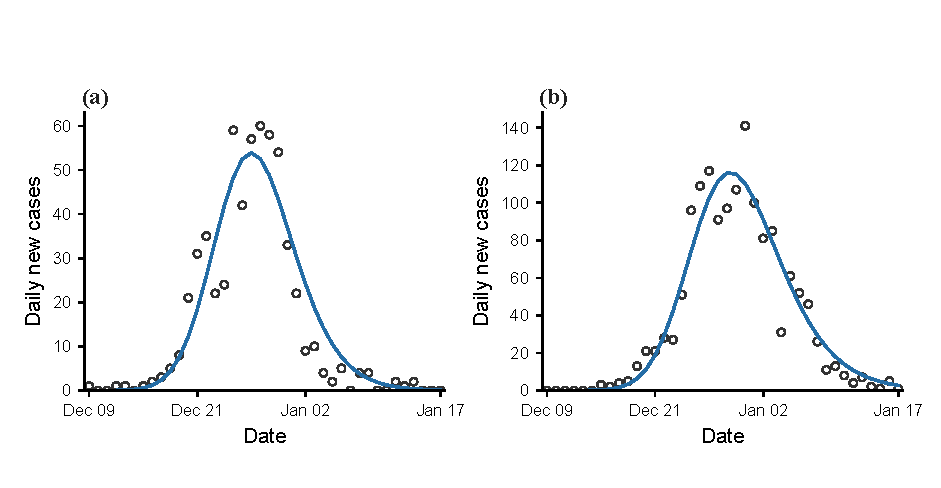
\includegraphics[width=\textwidth]{figures/layout_v5/xian_observed_fit.pdf}
\caption{西安疫情观测窗口内的日新增病例与 TDINN 重构。(a) 社区发现病例；(b) 隔离发现病例。点为观测值，实线取自三策略比较所用的同一 TDINN 轨迹，以相邻整数日累计量之差计算日新增。40 个日区间从 2021 年 12 月 9 日起算；本图用于拟合重构的比较，并非独立数据验证。}
\label{fig:xian:observed-fit}
\end{figure}

\subsection{西安参数下的隔离率阈值控制}
\label{sec:xian:threshold-scale}
本节采用西安人口及拟合传播参数，取代表性社区感染上限
\begin{equation}
\eta=0.002N=26{,}326.
\end{equation}
该阈值为设计情景，其医疗资源相关的量级参考见补充材料第\ref*{sec:sup:threshold-scale}节。各策略采用同一阈值比较，阈值变化的影响由后续敏感性分析考察。
按第~\ref{sec:s1}节，常规控制下临界易感人数 $S_c=\gamma N/[\beta c_0(1-q_0)]=2{,}974{,}125.41$；数值求得达到阈值时刻 $t_1=16.90$、启动点 $S^*=13{,}020{,}440.75$。阈值控制期由理论开环控制 $q_c(t)=1-\gamma N/[\beta c_0 S(t)]$（其中 $S(t)=\bar S+(S^*-\bar S)e^{-c_0\eta(t-t_1)/N}$，$\bar S=\gamma N(1-\beta)/(\beta c_0)$）维持 $I(t)\equiv\eta$，解除时刻
\[
t_2=t_1+\frac{N}{c_0\eta}\ln\frac{S^*-\bar S}{S_c-\bar S}\approx101.97,
\]
控制时长约 $85.07$ 天；启动隔离率 $q_c(t_1)=0.8454$，终点 $q_c(t_2)=q_0=0.3230$。阈值控制阶段最大数值偏差约为 $1.35\times10^{-6}$。

\subsection{比较指标与三策略数值结果}
三类策略均计算至各自的动态清零时刻，即 $I(t)$ 超过 $1$ 后再次下降至 $1$ 的时刻。成本采用第~\ref{sec:cost}~节的定义，权重为 $w_c=1,w_q=2$：TDINN 从初始时刻积分至清零，阈值控制仅在 $[t_1,t_2]$ 内产生额外成本，常规控制的额外成本为零。

图\ref{fig:xian:strategy-process}给出三类策略下的感染、总累计感染、有效再生数与控制轨迹，主要指标列于表\ref{tab:xian_summary}。

\begin{figure}[htbp]
\centering
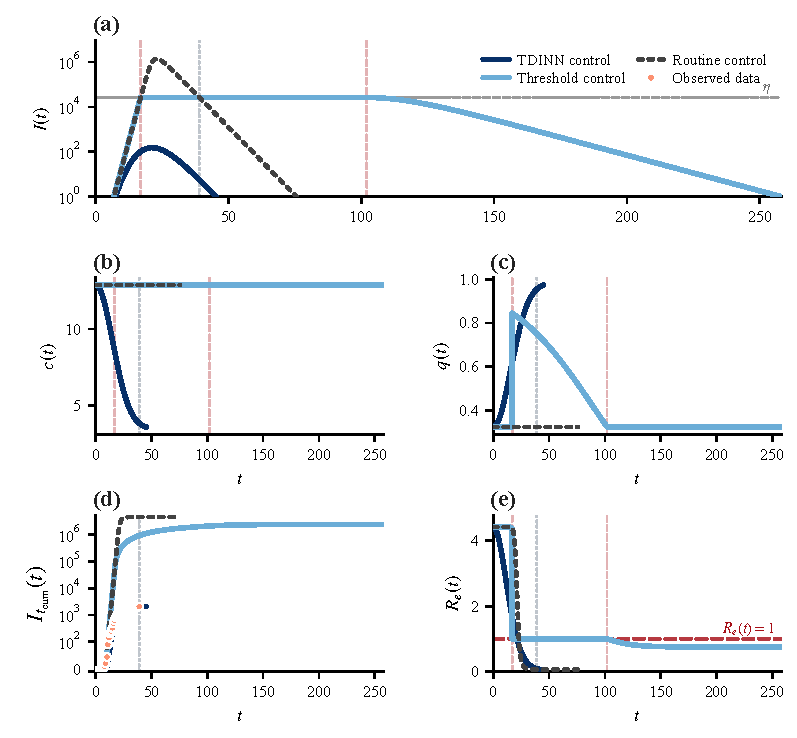
\includegraphics[width=135mm]{figures/layout_v5/xian_strategy_process.pdf}
\caption{$\eta=0.002N$ 时三策略的全过程比较。(a) 社区感染者人数 $I(t)$；(b) 接触率 $c(t)$；(c) 隔离率 $q(t)$；(d) 总累计感染 $\Itcum(t)$；(e) 有效再生数 $R_e(t)$。各轨迹分别画至自身的动态清零时刻，横轴使用同一时间原点，$t$ 的单位为天。(a) 为对数纵轴；(d) 为对称对数纵轴（线性区阈值为 $100$ 人），散点为观测累计量；(e) 的水平虚线为 $R_e=1$。浅红色竖虚线标记控制启动与解除，灰色竖点线标记观测窗口结束。}
\label{fig:xian:strategy-process}
\end{figure}

\begin{table}[htbp]
\centering\small
\setlength{\tabcolsep}{3.5pt}
\renewcommand{\arraystretch}{1.25}
\begin{threeparttable}
\caption{西安参数下三种策略的感染结局与干预指标}
\label{tab:xian_summary}
\begin{tabular*}{\linewidth}{@{\extracolsep{\fill}}lS[table-format=7.0]S[table-format=7.0]S[table-format=3.2]S[table-format=2.4]@{}}
\toprule
策略 & {\shortstack{社区感染峰值\\（人）}} & {\shortstack{总累计感染\\（人）}} & {\shortstack{动态清零时间\\（d）}} & {$J$（d）}\\
\midrule
TDINN 控制 & 153 & 2106 & 45.29 & 49.3894\\
隔离率阈值控制 & 26326 & 2377943 & 258.10 & 40.7686\\
常规控制 & 1377552 & 4587183 & 75.57 & 0.0000\\
\bottomrule
\end{tabular*}
\begin{tablenotes}[flushleft]\footnotesize
\item 注：$\eta=0.002N$ 为设计情景；各策略沿用原文规定的动态清零终点；人数四舍五入至整数。用于后续比较的 TDINN 参照为峰值152.55、总累计2105.63、清零时间45.29 d、$J=49.39$。$J$ 为二次加权积分，不由线性指标 $J_c,J_q$ 直接加总。阈值策略的启动、解除与控制时长分别为 $16.90$、$101.97$、$85.07$ d。
\end{tablenotes}
\end{threeparttable}
\end{table}


采用全市人口及 $\eta=0.002N$ 时，阈值控制将社区感染峰值限制为 $26{,}326$，阈值控制持续约 $85.07$ 天，动态清零时间约为 $258.10$ 天，总累计感染约为 $2.38\times10^6$。TDINN 重构的峰值和累计感染分别约为 $153$ 和 $2106$。阈值控制的二次加权成本为 $40.77$，低于 TDINN 的 $49.39$，但感染峰值、累计感染和清零时间均较大。后文采用更精确的 TDINN 参照值 $I_{\rm peak}^{\rm T}=152.55$、$\Itcum^{\rm T}=2105.63$ 和 $J^{\rm T}=49.39$。

有效再生数为 $R_e(t)=\beta c(t)(1-q(t))S(t)/(\gamma N)$。常规控制下 $R_e(0)\approx4.43$，感染人数初期快速增长；TDINN 同时降低接触率并提高隔离率，使 $R_e$ 较快降至 $1$ 以下；阈值控制则在阈值控制期保持 $R_e=1$，待 $S$ 下降至 $S_c$ 后恢复常规隔离率，感染人数才开始下降。因此，较低的加权成本在这里伴随着更长的感染持续时间和更高的累计感染。

% BEGIN JOINT_EXTRA:xian
在同一全市人口、未取整拟合初值及 $\eta=0.002N$ 下，第\ref{sec:joint:compare-numerics}节又比较了四种阈值分配（表\ref{tab:joint:compare}）。类内最小成本从仅隔离的 $40.7686$ 降至 $38.0209$，控制时长由 $85.07$ 延长至 $108.81$ d，总累计新增感染由约 $2.3779\times10^6$ 增至 $2.5348\times10^6$。相对变化分别约为成本 $-6.7\%$、控制时长 $+27.9\%$、总累计新增感染 $+6.6\%$。因此，这里的成本降低不伴随感染指标同时改善。TDINN 仍为另一终止任务下的外部参照，不属于固定启动状态、感染平台和退出状态的四策略比较类，也不据此宣称它已被联合阈值策略支配。
% END JOINT_EXTRA:xian

\subsection{阈值 \texorpdfstring{$\eta$}{eta} 的敏感性}
取 $\eta/N\in\{0.0001,0.0002,0.0005,0.001,0.0015,0.002,0.003,0.004,0.005,0.0075,0.01\}$，结果见表~\ref*{tab:sup:eta} 和图~\ref{fig:xian_eta_sens}。这些取值覆盖代表性阈值及其两侧的范围，用于比较不同设计情景。在这一范围内，有
\[
\eta\downarrow\ \Rightarrow\ t_1\downarrow,\qquad \Delta t\uparrow,\qquad J\uparrow,\qquad t_{\rm end}\uparrow.
\]
当 $\eta/N$ 从 $0.01$ 降至 $0.0001$ 时，启动时间仅由 $18.55$ 天提前至 $13.92$ 天，控制持续时间却由 $16.61$ 天增加至 $1710.66$ 天，动态清零时间达到 $2209.55$ 天。降低阈值减慢了阈值控制期的易感者减少过程，其对持续时间的影响远大于对启动时间的影响。


\begin{figure}[htbp]
    \centering
    \includegraphics[width=0.7\textwidth]{xian_eta_sensitivity.pdf}
    \caption{西安参数下控制指标随 $\eta/N$ 的变化。(a) 启动隔离率；(b) 加权成本；(c) 累计感染；(d) 控制持续时间与动态清零时间。水平线为 TDINN 参照值。(d) 中 TDINN 的控制时长和清零时间均为 $45.29$ d，前者为干预持续时间，后者为从共同时间原点起算的终点，数值相同并不表示两个定义相同。}
    \label{fig:xian_eta_sens}
\end{figure}

\FloatBarrier
\subsection{接触率 \texorpdfstring{$c_0$}{c0} 与阈值 \texorpdfstring{$\eta$}{eta} 的联合变化}
图~\ref{fig:xian_heatmaps} 给出 $(\eta,c_0)$ 平面上的控制持续时间、清零时间、累计感染和成本。两条参照线分别为设计情景 $\eta=0.002N=26326$ 和 TDINN 峰值 $\eta=I_{\rm peak}^{\rm T}=152.55$。

在西安全市人口设定（$N=13\,163\,000$，$c_0=12.8872$）下，由控制时长闭式
\[
\Delta t=\frac{N}{c_0\eta}\ln\frac{S^{*}-\bar S}{S_c-\bar S}
\]
有$\eta=0.002N=26326$ 时 $\Delta t\approx85$ 天；$\eta=152.55$ 时，$S^{*}\approx1.3162\times10^{7}$、对数因子约为 $2.205$，从而
\[
\Delta t(\eta=152.55)\approx1.48\times10^{4}\ \text{d}\approx 40.5\ \text{年}.
\]
规定退出状态也限制了累计感染。将本节参数代入命题\ref{prop:exit-infection-lower-bound}，得
\[
\Itcum(t_2)\ge\beta(S_0-S_c)\approx1.53\times10^6.
\]
因此，在本节全市人口及传播参数下，任何达到 $S=S_c$ 的策略都不能同时达到约 $2106$ 的累计感染参照。联合分配可能降低阈值控制类内的强度成本，但不能解除这个由退出目标造成的感染下界；这个结论也不排除提前消除传播或采用其他退出目标的策略。

这一时长是模型在固定参数和全市人口假设下的外推结果。由时间尺度 $N/(c_0\eta)$ 可见，较大的易感人群和较低的感染阈值会延长阈值控制期。在观测期累计病例约为 $2050$ 的拟合中，$S(t)\approx N$；但阈值策略需要持续至 $S=S_c$，因此其时间估计对人口规模尤为敏感。下一节考察不同有效混合人口下的结果。

\begin{figure}[htbp]
    \centering
    \includegraphics[width=0.8\textwidth]{xian_heatmaps.pdf}
    \caption{西安参数下 $(\eta,c_0)$ 平面上的控制指标。(a) 控制持续时间；(b) 动态清零时间；(c) 累计感染；(d) 加权成本。竖直参照线分别表示 TDINN 社区感染峰值 $\eta=152.55$ 和设计阈值 $\eta=26326$，等值线表示各指标的水平。}
    \label{fig:xian_heatmaps}
\end{figure}


\FloatBarrier

